\begin{frame}
    \vspace{-1cm}
    \centering
    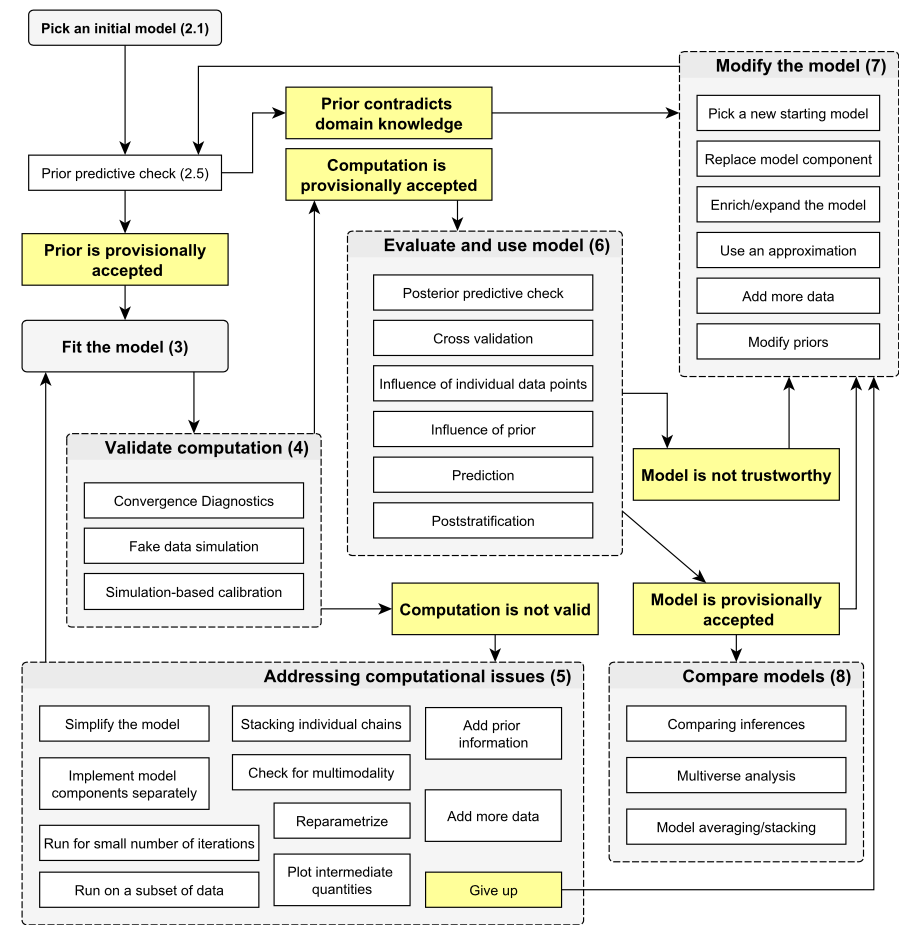
\includegraphics[width=0.75\linewidth]{../graphics/workflow}

    \scriptsize{Source: Gelman et al. (2020)}
\end{frame}

\begin{frame}{Iterative model improvement}
    \begin{enumerate}
        \item Initial models
        \item Priors on coefficients and scale parameters
        \item (Variable selection)
        \item Redefining the random effect
        \item Adding area-level spatial correlation
        \item Model comparison
    \end{enumerate}
\end{frame}

\begin{frame}{Initial model 1: Log-shift transformation}
    Like the model from \cite{morelli_hierarchical_2021}, but with full Bayesian inference on the shift term
    \begin{equation}
        \begin{split}
            p(y^*|\boldsymbol \beta, u_d, \sigma_e, \nu)   =        \text{Student}&(\log(y_{di} + \lambda)| \boldsymbol{x'}_{di} \boldsymbol \beta + u_d,\ \sigma_e\ , \nu)\cdot \frac 1 {(y_{di} + \lambda)}, \\
            u_d | \sigma_u & \sim \mathcal N(0, \sigma_u),\ d = 1, ..., D \\
            \beta_k & \sim \mathcal N(0, 0.5),\ k = 1, ..., K\\
            \sigma_u & \sim Ga(2, 0.75), \\
            \sigma_e & \sim Ga(2, 0.75), \\
            \nu & \sim Ga(2, 0.1), \\
            S(y^*) & \sim \mathcal N(0, 0.01),\\
        \end{split}
        \label{eq:trafo_hb}
    \end{equation}
\end{frame}

\begin{frame}{Initial model 1: Tightness of the prior on skewness}

    \begin{columns}
        \begin{column}{0.32\textwidth}
            \includegraphics[width=\linewidth]{../graphics/log_shift/bad_skewness}

            $S(y^*) \sim \mathcal N (0, 0.1)$
        \end{column}



        \begin{column}{0.32\textwidth}
            \includegraphics[width=\linewidth]{../graphics/log_shift/mid_skewness}

            $S(y^*) \sim \mathcal N (0, 0.01)$
        \end{column}


        \begin{column}{0.32\textwidth}
            \includegraphics[width=\linewidth]{../graphics/log_shift/gb2_skewness}

            $S(y^*) \sim \mathcal N (0, 0.001)$
        \end{column}

    \end{columns}
    \vspace{1cm}
    \textbf{Too wide}: unrealistic values and computational problems
    \vspace{0.5cm}

    \textbf{Too tight}: overfitting
\end{frame}

\begin{frame}
    \vspace{-0.5cm}
    \centering
    \includegraphics[width=0.85\linewidth]{../graphics/log_shift/logscale_smp_}

    \scriptsize{Posterior predictive check for log-scale scenario}

    \includegraphics[width=0.85\linewidth]{../graphics/log_shift/gb2_smp_}

    \scriptsize{Posterior predictive check for GB2 scenario}

    \includegraphics[width=0.85\linewidth]{../graphics/log_shift/pareto_smp_}

    \scriptsize{Posterior predictive check for Pareto scenario}

\end{frame}

\begin{frame}{Initial model 2: Skewed likelihoods}
    As an alternative model with skewed likelihoods were estimated:
    \begin{itemize}
        \item Skew-normal
        \item exGaussian
        \item Lognormal
        \item Gamma (log link)
        \item Gamma (softplus link)
    \end{itemize}
\end{frame}

\begin{frame}{Initial model 2: Skewed likelihoods}
    Additive likelihoods did not work well in the log-scale scenario

    \begin{columns}
        \begin{column}{0.49\textwidth}
            \centering
            \includegraphics[width=\linewidth]{../graphics/skewed_likelihood/single_graphs/skewnormal_logscale}

            Skew-normal
        \end{column}

        \begin{column}{0.49\textwidth}
            \centering
            \includegraphics[width=\linewidth]{../graphics/skewed_likelihood/single_graphs/exgaussian_logscale}

            exGaussian
        \end{column}
    \end{columns}

\end{frame}

\begin{frame}
    \vspace{-0.5cm}
    \scriptsize{The gamma log link had the best results of all the skewed likelihoods}
    \centering
    \includegraphics[width=0.8\linewidth]{../graphics/skewed_likelihood/gamma_log/logscale_smp_gamma_log}

    \scriptsize{Posterior predictive check for log-scale scenario}

    \includegraphics[width=0.8\linewidth]{../graphics/skewed_likelihood/gamma_log/gb2_smp_gamma_log}

    \scriptsize{Posterior predictive check for GB2 scenario}

    \includegraphics[width=0.8\linewidth]{../graphics/skewed_likelihood/gamma_log/pareto_smp_gamma_log}

    \scriptsize{Posterior predictive check for Pareto scenario}

\end{frame}

\begin{frame}{Defining priors on coefficients}
    \begin{itemize}
        \item In the log-shift model, coefficient are approximately percentage changes
        \item A change of more than 30\% for an additional unit seems excessive
        \item Coefficient prior is set to $\beta_k \sim \mathcal N(0, 0.2)$
    \end{itemize}
\end{frame}

\begin{frame}{Defining priors on scale parameters}
    \begin{itemize}
        \item $\sigma_e$ is not the standard deviation for a Student distribution
        \item The variance is defined as $\sigma^2 = \sigma_e^2\frac {\nu} {\nu -2}$
        \item $\sigma_e$ is redefined as $\sigma_e = \sigma \sqrt{\frac{\nu -2}{\nu}}$
        \item The gamma prior $Ga(2, a)$ is now placed on $\sigma_u$ and $\sigma$
        \item The rate parameter $a$ is determined with prior predictive checks
    \end{itemize}
\end{frame}

\begin{frame}{Prior predictive checks: scale prior}

    \centering
    Original scale prior: $Ga(2, 0.75)$
    \includegraphics[width=0.8\linewidth]{../graphics/prior_predictive_checks/prior_check_gb2_start}
\end{frame}

\begin{frame}{Prior predictive checks: scale prior}
    \centering
    Wide scale prior: $Ga(2, 0.01)$
    \includegraphics[width=0.8\linewidth]{../graphics/prior_predictive_checks/prior_check_gb2_wide}
\end{frame}

\begin{frame}{Prior predictive checks: scale prior}
    \centering
    Tight scale prior: $Ga(2, 7)$
    \includegraphics[width=0.8\linewidth]{../graphics/prior_predictive_checks/prior_check_gb2_tight}
\end{frame}

\begin{frame}{Full model}
    \vspace{-0.5cm}
    \begin{equation*}
        \begin{split}
            p(y_{di}^* |\boldsymbol \beta, u_d, \sigma_e, \nu)   = \text{Student}&(\log(y_{di} + \lambda)| \boldsymbol{x'}_{di} \boldsymbol \beta + u_d,\ \sigma_e\ , \nu)\cdot \frac 1 {(y_{di} + \lambda)}, \\
            u_d | \sigma_u & \sim \mathcal N(0, \sigma_u),\ d = 1, ..., D \\
            \beta_0 & \sim \mathcal N (0, 5),\\
            \beta_k & \sim \mathcal N(0, 0.2),\ k = 1, ..., K\\
            \tilde \nu & \sim Ga(2, 0.1), \\
            \nu & = \tilde \nu + 2,\\
            \sigma_u & \sim Ga(2, 7), \\
            \sigma & \sim Ga(2, 7), \\
            \sigma_e & = \sigma \sqrt{\frac{\nu - 2}{\nu}},\\
            S(y^*) & \sim \mathcal N(0, 0.01)\\
        \end{split}
        \label{eq:trafo_coef_var}
    \end{equation*}
\end{frame}

\begin{frame}{Redefining the random effect}
    \begin{itemize}
        \item Municipalities are an arbitrary division
        \item Municipalities are not taken into account in the survey design
        \item Better idea: use the stratification in the survey design
    \end{itemize}
\end{frame}

\begin{frame}{Redefining the random effect}
    \begin{itemize}
        \item Problem: survey and census have different stratification coding
        \item Solution: Use 5 indicator variables to approximate the stratification
        \item The combination of these 5 indicators results in 32 domains
    \end{itemize}
\end{frame}

\begin{frame}{Redefining the random effect}
    \begin{itemize}
        \item Advantage: no out-of-sample domains = less uncertainty
        \item Model with redefined domain has better predictive power
        \item Monte Carlo samples $\implies$ random effect and municipality do not have to coincide
    \end{itemize}
\end{frame}

\begin{frame}{Spatial Correlation}
    \begin{itemize}
        \item Complete independence of domain is highly unlikely
        \item LKJ prior
        \item SAR prior \cite{chung_bayesian_2020}
    \end{itemize}
\end{frame}

\begin{frame}{Spatial Correlation: LKJ prior}
    \begin{itemize}
        \item Prior on all possible correlation matrices
        \item The covariance matrix $\Sigma$ can be decomposed as $\Sigma = \sigma_u^2\Omega$
        \item LKJ prior is defined as: $p(\Omega|\eta) \propto \det(\Omega)^{\eta - 1}$
        \item Higher $\eta$ puts more weight on matrices similar to the identity matrix
    \end{itemize}
\end{frame}

\begin{frame}{Spatial Correlation: LKJ prior}
    \vspace{-1cm}
    \centering
    \includegraphics[width=0.85\textwidth]{../graphics/rand_intercept/lkj_corr_plot}
\end{frame}

\begin{frame}{Spatial Correlation: SAR prior}
    \begin{itemize}
        \item The $D\times D$ proximity matrix $W$ contains information on how close two domains are
        \item Here the Hamming distance is used
        \item Define $\widetilde W$ as the row-normalized version of of $W$
        \item SAR prior is defined on the precision matrix $\Omega$:
    \end{itemize}
    \begin{gather*}
        \Omega(\rho) = (I_D - \rho \widetilde W)'(I_D - \rho \widetilde W), ~~ \rho \in (-1, 1),\\
        u \sim \mathcal N(\boldsymbol{0}_D, \sigma_u^2 \Omega^{-1}),\\
        \rho \sim \mathcal U(-1, 1),
    \end{gather*}
\end{frame}

\begin{frame}{Spatial Correlation: SAR prior}
    \vspace{-1cm}
    \centering
    \includegraphics[width=0.85\textwidth]{../graphics/rand_intercept/sar_corr_plot}
\end{frame}

\begin{frame}{Spatial Correlation: Comparison}
    \begin{table}[ht]
        \centering
        \begin{tabular}{rrrrrrrrr}
            \hline
            & elpd$_{\text{loo}}$ diff. & S.E. diff. & elpd$_{\text{loo}}$ & S.E. elpd$_{\text{loo}}$  \\
            \hline
            Base & 0.00 & 0.00 & -14799.32 & 54.40  \\
            SAR & -0.07 & 0.24 & -14799.39 & 54.45  \\
            LKJ & -0.72 & 0.22 & -14800.05 & 54.40  \\
            \hline
        \end{tabular}
        %\caption{Comparison of LKJ, SAR and base specification with PSIS-LOO.}
        \label{tab:lkj_sar_base}
    \end{table}
\end{frame}

\begin{frame}{Model comparison with stacking}
    \begin{itemize}
        \item Stacking weights can be used to calculate a weighted average of predictions \cite{gelman_bayesian_2020}
        \item The weights are optimized jointly based on the elpd (predictive power)
        \item The weights can be used to gauge model heterogeneity
    \end{itemize}
    \begin{table}[ht]
        \begin{center}
            \begin{tabular}{rrrrrrr}
                \hline
                Mid skew. & Low skew. & High skew. & Base & LKJ & SAR \\
                \hline
                0.00 & 0.00 & 0.19 & 0.25 & 0.31 & 0.24 \\
                \hline
            \end{tabular}
        \end{center}
    \end{table}
\end{frame}